\section{Component Configurator}

The Component Configurator design pattern allows an application to link and unlink its componentn implementations at run-time without having to modify, recompile, or statically relink the application. Component Configurator further supports the reconfiguration of components into different application processes without having to shut down and re-start running processes.

\subsection{Kontext}

Ein System/eine Applikation in welcher Komponenten so flexibel und transparent wie möglich neugestartet, suspendiert oder wieder aufgeweckt werden muss.

\subsection{Problem}

Komponenten-basierte Applikationen müssen einen Mechanismus zur Verfügung stellen, um diese Komponenten in mehrere Prozesse aufteilen zu können (konfigurierbar).
Die Lösung zu diesem Problem ist durch 3 Bedingungen eingeschränkt:

\begin{itemize}
	\item Es sollte möglich sein, Implementationen von Komponenten an jedem Punkt im Lifecycle der Applikation zu ersetzen
	\begin{itemize}
		\item Modifikationen an einer Komponente dürfen nur minimale Auswirkungen auf andere Komponenten haben
		\item Auch das neustarten etc. einer Kopmonente darf nur minimale Auswirkungen auf andere Kompoenten haben
	\end{itemize}
	\item Entwickler eines Systems wissen meist nicht im Voraus, wie eine Komponente optimalerweise in Prozesse gesplittet werden sollte
	\begin{itemize}
		\item erste Konfigurationen von Komponenten können mit der Zeit suboptimal sein (Plattform upgrades, erhöhte Workloads etc.) und müssen neukonfiguriert werden
	\end{itemize}
	\item Das Konfigurieren, Initialisieren und Kontrollieren von Kopmonents (Administrative Tätigkeiten) müssen einfach und Komponenten-unabhängig sein
\end{itemize}

\subsection{Lösung}

Komponenten-Schnittstellen von der Implementation und Applikationen von der Konfiguration der Komponenten unabhängig machen.

\subsection{Struktur}

\begin{itemize}
	\item ein Komponenten-Interface definiert eine gleichartige Schnittstelle um diese zu Konfigurieren und Administrieren
	\item Konkrete Komponenten implementieren dieses Interface
	\item Ein Komponenten-Repository verwaltet alle konfigurierten Konkreten Komponenten
	\item Ein \emph{Component Configurator} verwendet das Komponenten-Repository um die neukonfiguration von Konkreten Komponenten zu verwalten/koordinieren
	\item Applikationen verwenden diese Interfaces um Komponenten zu administrieren
\end{itemize}

\subsubsection*{Klassendiagramm}


\begin{figure}[H]
	\centering
	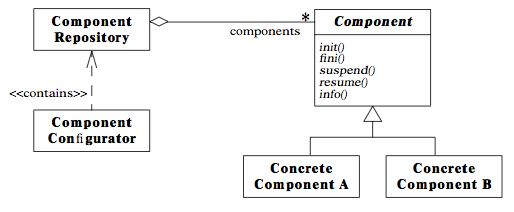
\includegraphics[width=\textwidth]{content/posa2/component-configurator/images/component-configurator-classdiagram.png}
	\caption{component configurator classdiagram}
\end{figure}


\subsubsection*{Sequenzdiagramm}


\begin{figure}[H]
	\centering
	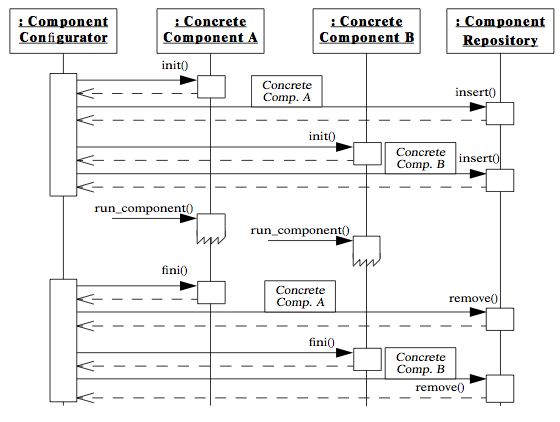
\includegraphics[width=\textwidth]{content/posa2/component-configurator/images/component-configurator-sequencediagram.png}
	\caption{component configurator sequencediagram}
\end{figure}


\subsubsection*{Zustandsdiagramm einer einzelnen Konkreten Komponente}


\begin{figure}[H]
	\centering
	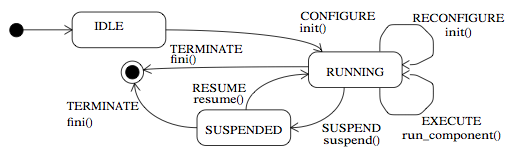
\includegraphics[width=\textwidth]{content/posa2/component-configurator/images/component-configurator-statediagram.png}
	\caption{component configurator statediagram}
\end{figure}


\subsection{Implementation}

Das Komponente-Interface kann entweder über Inheritance oder über Message Passing implementiert werden

\subsection{Vorteile}

\begin{itemize}
	\item Uniforme Konfiguration und Administration von Komponenten
	\item Zentralisierte Administration
	\item Modularität, Testbarkeit und Wiederverwendbarkeit von Komponenten
	\item Dynamische neukonfiguration
	\item Optimierung und Tuning während der Laufzeit möglich
\end{itemize}

\subsection{Nachteile}

\begin{itemize}
	\item Determinismus ist schwer nachzuvollziehen bis die Applikation vollständig konfiguriert ist
	\item Reduzierte Sicherheit und Verlässlichkeit
	\begin{itemize}
		\item Sicherheit weil sich Betrüger als Komponenten maskieren könnten
		\item Verlässlichkeit weil eine falsch konfigurierte Komponente die Ausführung der Komponente beeinträchtigen kann
		\begin{itemize}
			\item Auch weil eine Komponente crashen kann und die Zustandsinformationen die sie mit anderen Komponenten teilt beschädigen kann
		\end{itemize}
	\end{itemize}
	\item Erhöhter Runtime Overhead und Infrastruktur Komplexität
	\item Interfaces der Komponenten könnten zu tightly coupled oder zu komplex sein, um uniform ausgeführt zu werden
\end{itemize}

\subsection{Known Uses}

\begin{itemize}
	\item Windows NT Service Control Manager
	\item Device Drivers
\end{itemize}

\subsection{Prüfungsfragen}




